\documentclass[a4paper, 11pt]{article}
\usepackage{comment} % enables the use of multi-line comments (\ifx \fi) 
\usepackage{lipsum} %This package just generates Lorem Ipsum filler text. 
\usepackage{fullpage} % changes the margin
\usepackage{graphicx, wrapfig, subcaption, setspace, booktabs}
\usepackage{url}

\begin{document}
%Header-Make sure you update this information!!!!
\noindent
\large\textbf{Exploring delays in air travel in the United States} \hfill \textbf{Sara Arango-Franco} \\
\normalsize \url{github.com/sarangof/air-travel-USA/} 

\section*{Problem Statement}
The RITA \footnote{SIGLA} data set consists on records of airplane trips between airports in the United States since 1987. In this exercise I wondered about flight delays: how do they distribute geographically, how are they related with the relative importance of the most affected airports for domestic air transportation? 

A conversation with an airline schedule specialist made me wonder if it is true that carriers are extending scheduled flight duration in order to have a better on-time performance. 

\section*{Airports as a network}


Explanation: Network representation, etc.

Table: list of most important airports in terms of network centrality.


\begin{figure}[!ht]
  \caption{Arrival vulnerability (continental USA).}
  \label{m_days}
  \centering
    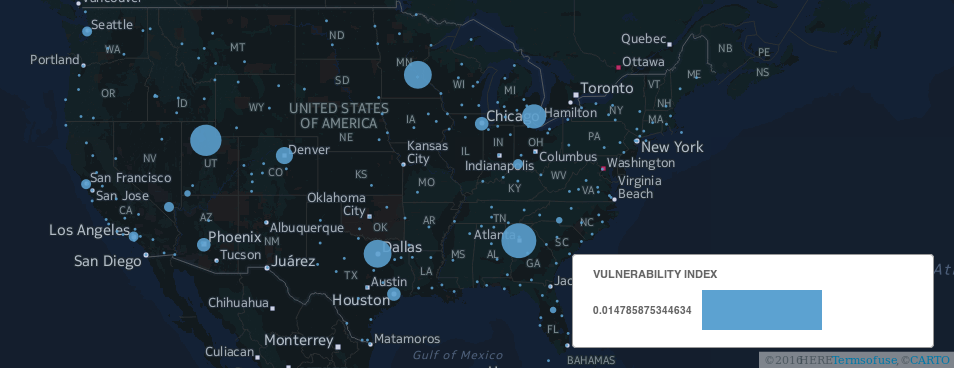
\includegraphics[width=\textwidth]{/home/saf537/Documents/Spotify/air-travel-USA/plots/arrival_vulnerability}
\end{figure}

\begin{figure}[!ht]
  \caption{Departure vulnerability (continental USA).}
  \label{m_days}
  \centering
    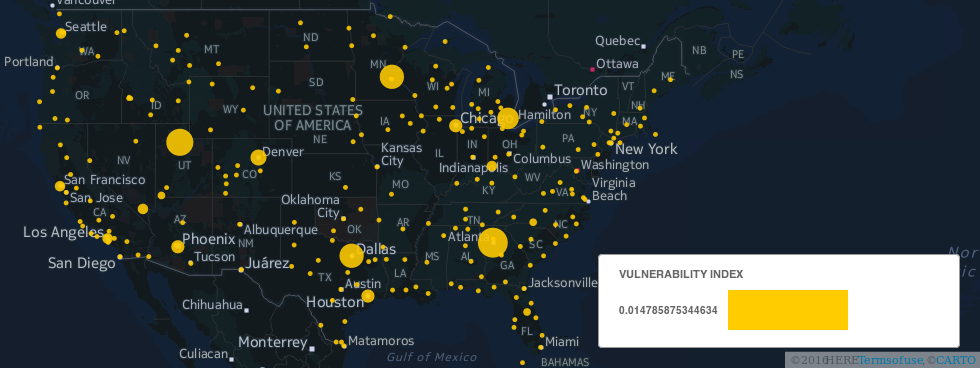
\includegraphics[width=\textwidth]{/home/saf537/Documents/Spotify/air-travel-USA/plots/departure_vulnerability}
\end{figure}


Table: list of most vulnerable airports in terms of arrivals

Table: list of most vulnerable airports in terms of departures

%\begin{figure}[!ht]
%  \caption{Missing days in the dataset.}
%  \label{m_days}
%  \centering
%    \includegraphics[scale=0.6]{/home/saf537/Documents/Spotify/air-travel-USA/plots/test}
%\end{figure}

\section*{Is on-time performance improving with time?}

Explanation of the aggregation that needed to take place: only comparable trips made sense.

plot: scheduling along the years.

plot: total delays along the years.


\begin{figure}[!ht]
  \caption{Scheduled trips length along the years in question.}
  \label{m_days}
  \centering
    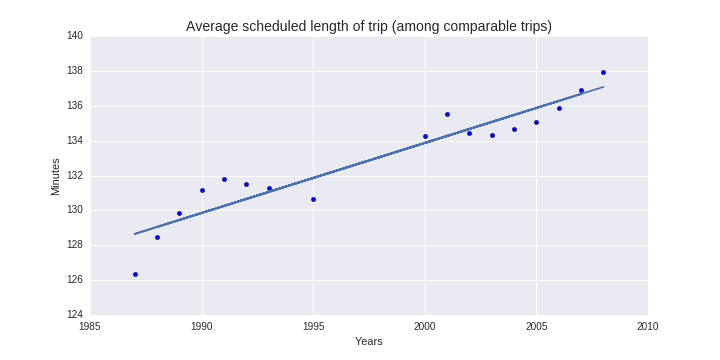
\includegraphics[width=\textwidth]{/home/saf537/Documents/Spotify/air-travel-USA/plots/sch_trips}
\end{figure}


\begin{figure}[!ht]
  \caption{Total delay along the years in question.}
  \label{m_days}
  \centering
    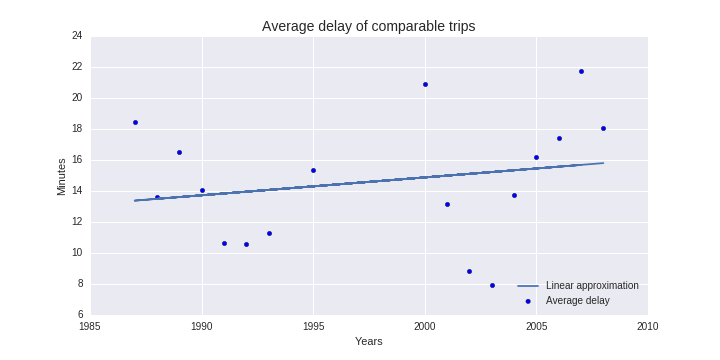
\includegraphics[width=\textwidth]{/home/saf537/Documents/Spotify/air-travel-USA/plots/del_trips}
\end{figure}

\section*{Comments and conclusions}

Clearly this is a biased metric because airports take both national and international flights.

Causality is not proven nor investigated in the last section.

% to comment sections out, use the command \ifx and \fi. Use this technique when writing your pre lab. For example, to comment something out I would do:
%  \ifx
%	\begin{itemize}
%		\item item1
%		\item item2
%	\end{itemize}	
%  \fi

\section*{Construction/Implementation}

\section*{Analysis \& Testing}


\section*{Final Evaluation}




\end{document}
